\documentclass[%
%draft,%
11pt,%
%oneside,%
twoside,%‡
%twocolumn,%
titlepage,%
%fleqn,%
%a4page,%
german,%
headsepline%
]{scrartcl}

\usepackage{lastpage}
\usepackage{geometry}
\usepackage{graphicx}
\usepackage[utf8]{inputenc}
\usepackage[ngerman]{babel}
\usepackage{lscape}
\usepackage[framemethod=TikZ]{mdframed}
\usepackage[most]{tcolorbox}
\usepackage{mymath}
\usepackage{units}
\usepackage{nicefrac}
\usepackage{pgf,tikz}
\usetikzlibrary{arrows}
\usepackage{colortbl}
\usepackage{hhline}
\usepackage{multirow}
\usepackage[extendedchars]{grffile}
\usepackage{caption}
\usepackage{multicol,calc}
\usepackage{blindtext}
\usepackage{pdfpages}
\usepackage{hyperref}
\usepackage{framed}
\usetikzlibrary{arrows}
\usetikzlibrary{positioning}
\usetikzlibrary{shadows}
\usepackage{pgfplots}
\pgfplotsset{compat=1.15}
\usepackage{mathrsfs}

\usepackage{ocg}
\usepackage{fontawesome}
\usepackage{xcolor}

\usepackage{marginnote}
\usepackage
%[draft]%
{qrcode}
\qrset{height=9ex}

\usepackage{longtable}
\usepackage{listings}
\usepackage{wrapfig}

\usepackage{fontawesome} % Oder FontAwesome, falls du ein Augensymbol aus einer
\definecolor{lightgray}{rgb}{0.7, 0.7, 0.7}
\newcommand{\faEyeLightGray}{\textcolor{lightgray}{\faEye}} % Custom command for the gray eye icon

\newcommand{\geogebralink}{\href{https://www.geogebra.org/calculator}{\texttt{geogebra.org}}}

% Command, um Tabellen-Spalten anzupassen
\newcommand{\spaltenheight}{\rule{0mm}{3ex}}
\newcommand{\spaltenwidth}{\rule{3cm}{0mm}}
\newcommand{\spaltensep}{\\[1ex]}
\doublerulesepcolor{white}
\definecolor{lightyellow}{rgb}{1,1,0.8}
\definecolor{Gray}{gray}{0.9}

\pagestyle{headings} % gemachte Einstellungen anwenden

% Farbig umrahmte Umgebung Satz
\definecolor{myblizzardblue}{HTML}{87CEEB}

\newcounter{satzz}[section]\setcounter{satzz}{0}
\renewcommand{\thesatz}{\arabic{section}.\arabic{satzz}}

\newenvironment{csatz}[1][]{%
    \refstepcounter{satzz}
 
    \ifstrempty{#1}%
    % if condition (without title)
    {\mdfsetup{%
        frametitle={%
            \tikz[baseline=(current bounding box.east),outer sep=0pt]
            \node[anchor=east,rectangle,fill=myblizzardblue]
            {\strut Satz~\thesatz};}
        }%
    % else condition (with title)
    }{\mdfsetup{%
        frametitle={%
            \tikz[baseline=(current bounding box.east),outer sep=0pt]
            \node[anchor=east,rectangle,fill=myblizzardblue]
            {\strut Satz~\thesatz:~#1};}%
        }%
    }%
% for both conditions
    \mdfsetup{%
        innertopmargin=10pt,linecolor=myblizzardblue,%
        backgroundcolor=whitesmoke,%
        linewidth=2pt,topline=true,%
        frametitleaboveskip=\dimexpr-\ht\strutbox\relax%
    }
 
\begin{mdframed}[]\relax}{%
\end{mdframed}}

% Farbig umrahmte Umgebung Theorem
 
\definecolor{mygraphblue}{HTML}{84B7E1}
\definecolor{whitesmoke}{HTML}{F5F5F5}

\newcounter{theo}[section]\setcounter{theo}{0}
\renewcommand{\thetheo}{\arabic{section}.\arabic{theo}}

\newenvironment{ctheo}[2][]{%
    \refstepcounter{theo}
 
    \ifstrempty{#1}%
    % if condition (without title)
    {\mdfsetup{%
        frametitle={%
            \tikz[baseline=(current bounding box.east),outer sep=0pt]
            \node[anchor=east,rectangle,fill=mygraphblue]
            {\strut Theorem~\thetheo};}
        }%
    % else condition (with title)
    }{\mdfsetup{%
        frametitle={%
            \tikz[baseline=(current bounding box.east),outer sep=0pt]
            \node[anchor=east,rectangle,fill=mygraphblue]
            {\strut Theorem~\thetheo:~#1};}%
        }%
    }%
% for both conditions
    \mdfsetup{%
        innertopmargin=10pt,linecolor=mygraphblue,%
        backgroundcolor=whitesmoke,%
        linewidth=2pt,topline=true,%
        frametitleaboveskip=\dimexpr-\ht\strutbox\relax%
    }
 
\begin{mdframed}[]\relax}{%
\end{mdframed}}

% Farbig umrahmte Umgebung Definition
 
 \definecolor{emerald}{HTML}{50C878}

\newcounter{deff}[section]\setcounter{deff}{0}
\renewcommand{\thedeff}{\arabic{section}.\arabic{deff}}

\newenvironment{cdef}[1][]{%
    \refstepcounter{deff}
 
    \ifstrempty{#1}%
    % if condition (without title)
    {\mdfsetup{%
        frametitle={%
            \tikz[baseline=(current bounding box.east),outer sep=0pt]
            \node[anchor=east,rectangle,fill=emerald]
            {\strut Definition~\thedeff};}
        }%
    % else condition (with title)
    }{\mdfsetup{%
        frametitle={%
            \tikz[baseline=(current bounding box.east),outer sep=0pt]
            \node[anchor=east,rectangle,fill=emerald]
            {\strut Definition~\thedeff:~#1};}%
        }%
    }%
% for both conditions
    \mdfsetup{%
        innertopmargin=10pt,linecolor=emerald,%
        backgroundcolor=whitesmoke,%
        linewidth=2pt,topline=true,%
        frametitleaboveskip=\dimexpr-\ht\strutbox\relax%
    }
 
\begin{mdframed}[]\relax}{%
\end{mdframed}}

% Farbig umrahmte Umgebung Achtung
 
 \definecolor{mygraphred}{HTML}{E26A6A}

\newcounter{merkee}[section]\setcounter{merkee}{0}
\renewcommand{\themerkee}{\arabic{section}.\arabic{merkee}}

\newenvironment{cachtung}[2][]{%
    \refstepcounter{merkee}
 
    \ifstrempty{#1}%
    % if condition (without title)
    {\mdfsetup{%
        frametitle={%
            \tikz[baseline=(current bounding box.east),outer sep=0pt]
            \node[anchor=east,rectangle,fill=mygraphred]
            {\strut Achtung};}
        }%
    % else condition (with title)
    }{\mdfsetup{%
        frametitle={%
            \tikz[baseline=(current bounding box.east),outer sep=0pt]
            \node[anchor=east,rectangle,fill=mygraphred]
            {\strut Achtung:~#1};}%
        }%
    }%
% for both conditions
    \mdfsetup{%
        innertopmargin=10pt,linecolor=mygraphred,%
        backgroundcolor=whitesmoke,%
        linewidth=2pt,topline=true,%
        frametitleaboveskip=\dimexpr-\ht\strutbox\relax%
    }
\begin{mdframed}[]\relax}{%
\end{mdframed}}

%\newtheorem{uebthm}{Übung}[section]
% Umgebung lsg mit dynamischer Referenzierung und Label
\newcommand{\concatueb}[1]{ueb:#1}% Definition für concatueb
\newcommand{\concatlsg}[1]{lsg:#1}% Definition für concatlsg

\newcounter{uebcounter}[section]
\renewcommand{\theuebcounter}{\thesection.\arabic{uebcounter}}  % Zählerformat: Abschnitt.Übung

% Definition einer Übungsumgebung mit dynamischen Labels
\newcommand{\uebh}[2]{%
 \refstepcounter{uebcounter} % Zählt den Übungscounter hoch
 \par\noindent\textbf{Übung \theuebcounter:}\label{\concatueb{#1}} % Label im Format "ueb:1"
    #2
    \hfill\hyperref[\concatlsg{#1}]{\faEyeLightGray}
    \vspace{\parskip}
}

\newenvironment{lsg}[1]{%
    \par\noindent\textbf{Notizen zu Übung \ref{\concatueb{#1}}.}%
    \label{\concatlsg{#1}}
}{%
    \par%
}

\newenvironment{uebenv}[1]{%
    \refstepcounter{uebcounter}
    \par\noindent\textbf{Übung \theuebcounter.}%
    \label{\concatueb{#1}}\hfill\hyperref[\concatlsg{#1}]{\faEyeLightGray}\par
}{%
    \par
}

\newcommand{\definition}[1]{\colorbox{emerald}{#1}}

\setlength{\parindent}{0pt}

\subject{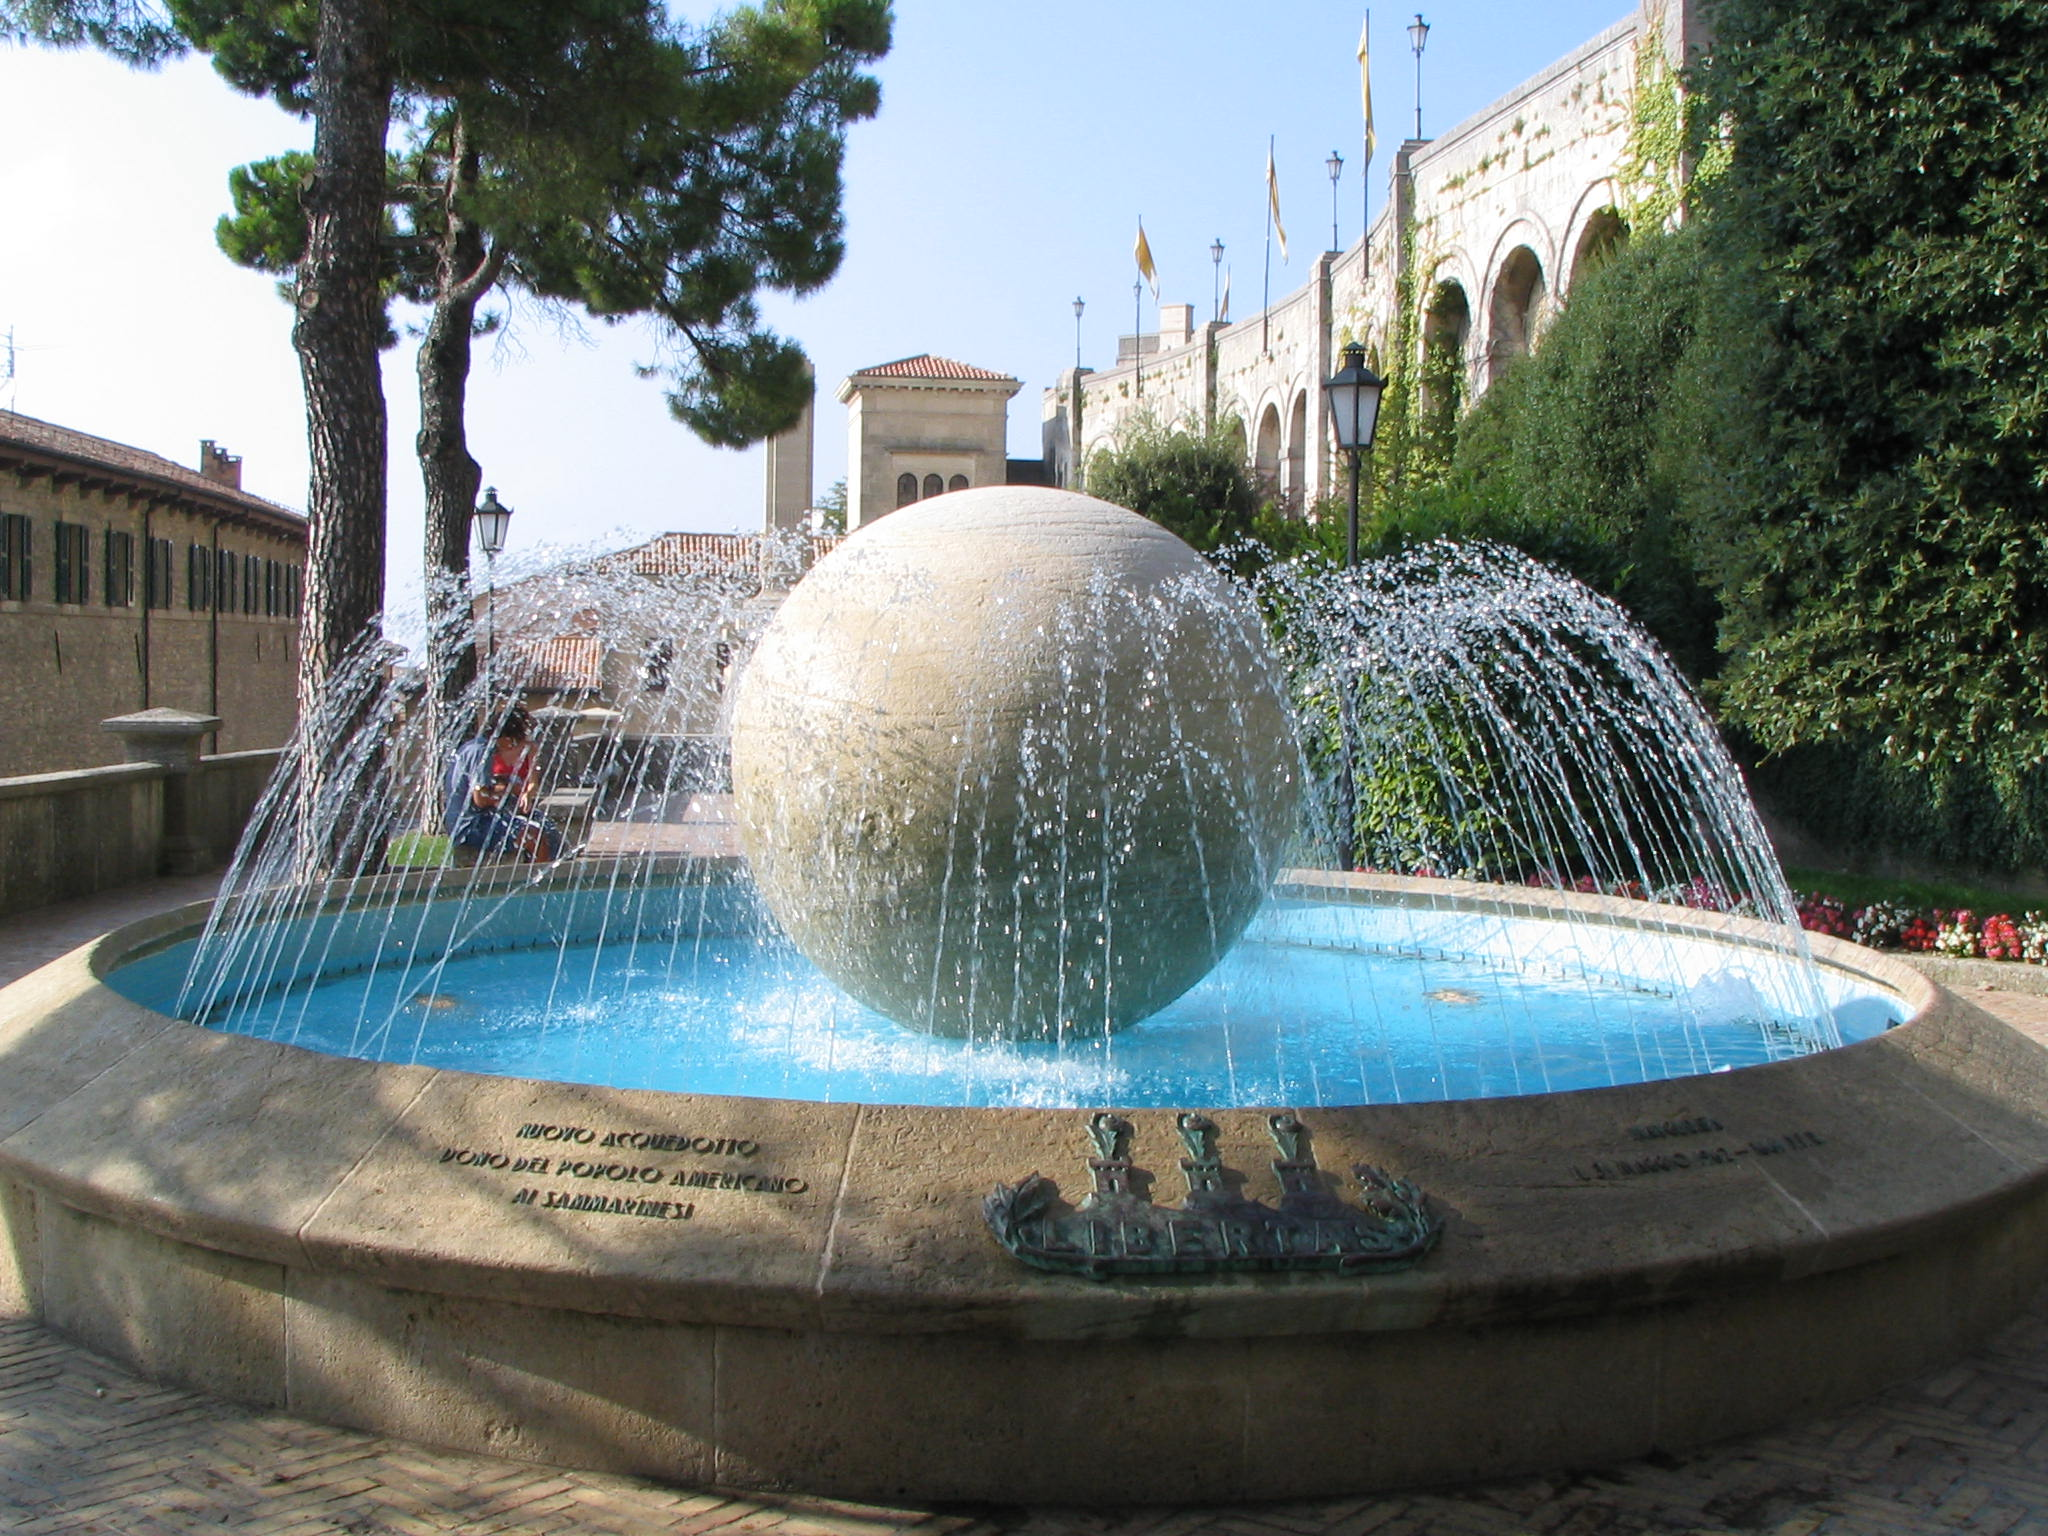
\includegraphics[width=0.618\textwidth]{pictures/springbrunnen.jpg}}
\title{Funktionentypen}
\subtitle{beyond linear}
\author{}
\date{}
\lowertitleback{

\includegraphics[height=1cm]{pictures/gymfmslerbermattlogo.eps}
\hfill%\copyright%
{\begin{tikzpicture}
  % Draw the rounded rectangle and clip the image to it
  \clip [rounded corners=5mm] (0,0) rectangle (1,1); % Adjust dimensions as needed
  \node at (0.5,0.5) {\includegraphics[width=1cm]{pictures/teacher_me_caricatur.png}}; % Adjust width and center image
\end{tikzpicture}}
}


\begin{document}
\maketitle
\tableofcontents
\cleardoublepage

\clearpage

\section{Exponentialfunktionen}

\subsection{Einleitung}
\begin{wrapfigure}{r}{0.3\textwidth}
  \begin{center}
    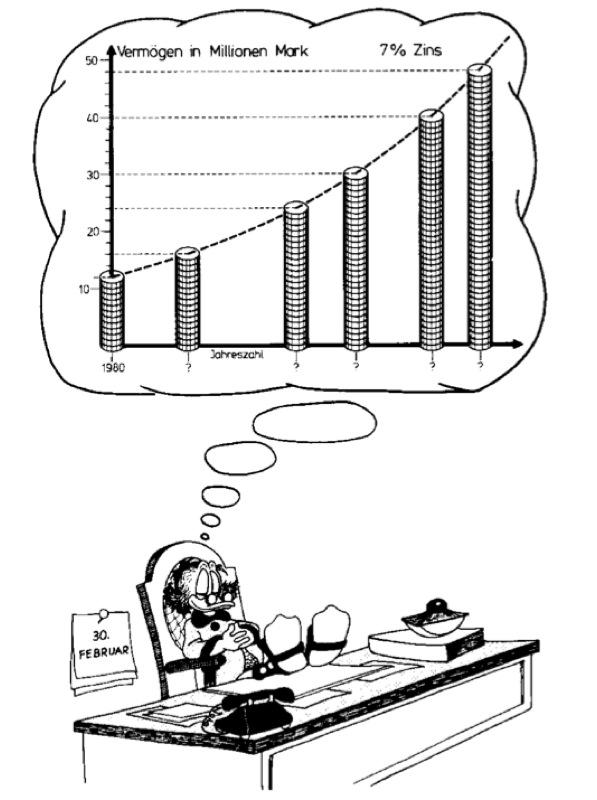
\includegraphics[width=0.2\textwidth]{pictures/dagobert}
  \end{center}
\end{wrapfigure}
Seit der Pandemie von SARS2 CoV19 im Jahr 2020 ist der Begriff des \emph{exponentiellen Wachstums} in aller Munde. Ein Beispiel aus einer Tageszeitung --- dem Tagesspiegel Ausgabe vom 12.3.21 --- fand ich hier:
    \href{https://www.tagesspiegel.de/wirtschaft/wie-exponentielles-wachstum-unser-leben-beeinflusst-4236517.html}{Wie exponentielles Wachstum unser Leben beeinflusst}
Dieser wichtige Typ Funktion soll nun in diesem Kapitel ergründet werden.

\begin{bsp}
Ein Schüler verbreitet zu Beginn der grossen Pause im Gymnasium Lerbermatt ein Gerücht. Alle Minuten erzählt ein Wissender einem Nicht-Eingeweihten das Gerücht. Wie lange dauert es, bis alle Schüler des Gymnasiums über das Gerücht in Kenntnis gesetzt worden sind?
\end{bsp}

Bei den Potenzfunktionen sind die Exponenten immer Konstanten, bei den Exponentialfunktionen ist die Basis konstant und der Exponent variabel.
\begin{cdef}[Exponentialfunktion]{}
Eine Funktion der Form
$$f(x)=b^x$$
mit $b\in\mR^+$ heisst \emph{Exponentialfunktion} zur Basis $b$.
\end{cdef}

\begin{bsp}
Anwendungen, die durch Exponentialfunktionen beschrieben werden sind:
\begin{itemize}
\item Ausbreitung von Krankheiten/Epidemien
\item Radioaktiver Zerfall
\item Zellvermehrung
\end{itemize}
\end{bsp}

\subsection{Graphen}
\uebh{}{
\label{uebgraphen}
Zeichne in dasselbe Koordinatensystem die Graphen
der Funktionen\\

(a) $2^x$, $3^x$, $2.7^x$ (b) $4^x$, $\left(\frac{1}{4}\right)^x$, $10^x$
}

\uebh{}{
Vergleiche das Verhalten (insbesondere das Wachstum) der beiden Funktionen
$$p(x)=x^2\q\text{und}\q e(x)=2^x$$
}

\begin{bem}
Der Graph der Exponentialfunktionen
$$f(x)=b^x$$
liegt oberhalb der x-Achse und geht durch den Punkt $\point{0}{1}$. Für $b>1$ ist der Graph steigend ($f$ monoton wachsend) und die negative $x$-Achse Asymptote; für $0<b<1$ ist der Graph fallend ($f$ monoton fallend) und die positive $x$-Achse Asymptote.
\end{bem}

\begin{csatz}[Wachstum- \& Zerfall]{}
Die Kurven mit den Gleichungen $y=b^x$ und $y=\left(\frac{1}{b}\right)^x$ liegen symmetrisch zueinander bezüglich der y-Achse.
\end{csatz}

\begin{proof}[Beweis]
Übung.
\end{proof}

\uebh{}{
Berechne für die Funktionen der Übung \ref{uebgraphen} die durchschnittlichen ¨Änderungsraten über den Intervallen $[0,1]$ und $[-1,0]$.
}

\uebh{}{
Zeichne den Graphen von $f(x)=2^x$ in ein Koordinatensystem.
\begin{enumerate}[a)]
\item Verschiebe den Graphen in positiver x-Richtung
um 3 Einheiten.
\item Spiegele den Graphen an der x-Achse.
\item Verschiebe den Graphen in negativer y-Richtung
um 4 Einheiten.
\item Spiegele den Graphen an der y-Achse.
\item Spiegele den Graphen am Ursprung des Koordinatensystems.
\end{enumerate}
Geben Sie jeweils die Gleichung der Bildkurve an.
}

\begin{figure}
  \begin{center}
    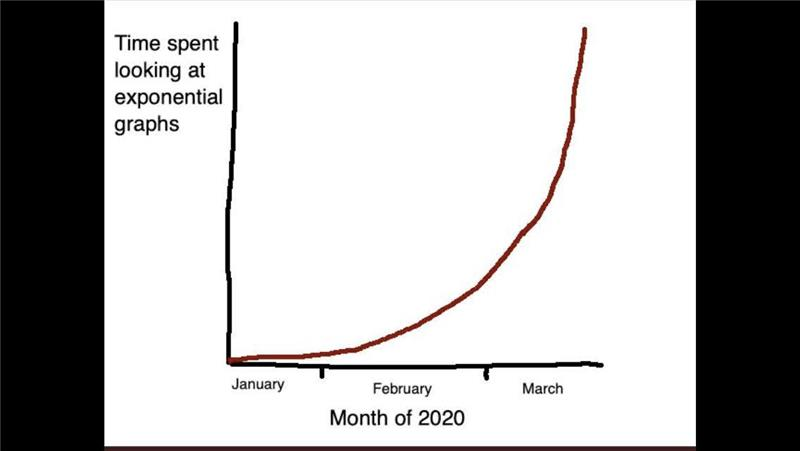
\includegraphics[width=0.618\textwidth]{pictures/exponentialgraphs.jpg}
    \caption{Joke During SARS2-CoV19 Lockdown in 2020}
  \end{center}
\end{figure}

\uebh{}{
Es sei
$$f(x)=b^x\text{ und }g(x)=a\cdot b^x.$$
Der Punkt $P$ liegt auf dem Graphen von $f$. Berechne $b$ für
\begin{enumerate}[a)]
\item $P=\point{1.5}{27}$
\item $P=\point{4}{9}$
\end{enumerate}
Die Punkte $R$ und $Q$ liegen auf dem Graphen von $g$. Berechne $a$ und $b$ für
\begin{enumerate}[a)]
\setcounter{enumi}{2}
\item $R\point{0}{2}, Q\point{2}{18}$
\item $R\point{-2}{20}, Q=\point{3}{\frac{5}{8}}$
\end{enumerate}
}

\subsection{Wachstum und Zerfall}
Die Exponentialfunktionen spielen bei der Beschreibung von zeitabhängigen Wachstums- und Zerfallserscheinungen eine ausserordentlich wichtige Rolle.
\begin{cdef}[Exponentialfunktion allgemein]{}
  Ist $t$ die Masszahl der Zeit, so bezeichnet man die Funktion
$$f(t)=ab^t$$
für $b>1$ als \emph{exponentielle} Wachstumsfunktion, für $0<b<1$
als exponentielle Zerfallsfunktion.
\end{cdef}
\begin{bem}
Zum Zeitpunkt $t=0$ gilt
$$f(0)=ab^0=a.$$
Also ist $(0|a)$ der Schnittpunkt mit der $y$-Achse, und man nennt $a$ den Anfangswert von $f$. Der Parameter $b$ ist ein Mass für das Wachstum bzw. den Zerfall und wird deshalb Wachstums- bzw. Zerfallsfaktor genannt.
\end{bem}

\uebh{}{
Bei einer Bakterienkultur ohne Raum- und Nahrungsmangel wächst die Individuenzahl exponentiell. Um 8 Uhr waren es 2300 und um 12 Uhr 36800 Individuen.
\begin{enumerate}[a)]
\item Nimm 2300 als Anfangswert an und ermittle den Wachstumsfaktor $b$. Wie lautet demnach die entsprechende Wachstumsfunktion?
\item Welches ist die Individuenzahl um 9 Uhr, um 11 Uhr, um 13.30 Uhr?\label{bakterienb}
\end{enumerate}
}

\uebh{}{
Ein Waldbestand, in dem kein Holz geschlagen wird, wächst exponentiell. Er beträgt heute $\unit[72\,342]{m^3}$, vor zwölf Jahren betrug er $\unit[48\,228]{m^3}$.
\begin{enumerate}[a)]
\item Wie hoch war der Waldbestand vor fünf Jahren?
\item Wie hoch wird er heute in sieben Jahren sein?
\end{enumerate}
}

\uebh{}{
In einer Bakterienkultur ist $$f(t) =10^4 \cdot 2^\frac{t}{2}$$ die Anzahl der Bakterien zum Zeitpunkt $t$. In welcher Zeitspanne $\Delta t$ verdoppelt, vervierfacht, verachtfacht sich die Anzahl?
}

\begin{bem}
In der Praxis werden viele Wachstumsprozesse dadurch beschrieben, dass man neben dem Startwert $a$ noch die jährliche Zunahme der betrachteten Grösse in Prozenten angibt. Man denke einfach an die wohlbekannte Zinseszinsrechnung.
\end{bem}

\begin{bsp}
Es sei $f(0)=a=10000$ die Anzahl der Einwohner einer Stadt, deren jährliches Wachstum $2\%$ beträgt. Nach einem Jahr hat die Stadt $$f(1)=f(0)+0.02\cdot f(0)=f(0)\cdot(1+0.02)=10200$$ Einwohner. Nach zwei Jahren sind es
$$f(2)=f(1)\cdot(1+0.02)=f(0)\cdot(1+0.02)^2$$ Einwohner und analog nach $t$ Jahren
$$f(t)=10000\cdot1.02^t$$ Einwohner.
\end{bsp}

\uebh{}{
Vom Jahr 1875 zum Jahr 1985 ist die Wohnbevölkerung der Schweiz von 2\,750\,300 auf 6\,455\,900 angewachsen. Wieviel Prozent betrug die jährliche Zunahme, wenn man annimmt, dass die Bevölkerung von Jahr zu Jahr gleich viele Prozent zugenommen hat?
%In Wirklichkeit verlief die Zunahme unregelmässig; siehe dazu Tabelle \ref{tab:bevoelkerung} auf Seite \pageref{tab:bevoelkerung}.
\definecolor{Gray}{gray}{0.9}
%\definecolor{darkgreen}{rgb}{0,0.4,0}
\definecolor{lightyellow}{rgb}{1,1,0.8}
%\arrayrulecolor{darkgreen}
%\doublerulesepcolor{black}
\begin{table}
\small
\begin{center}
\begin{tabular}{|c|c|}
\hline
\rowcolor{Gray}\spaltenheight Jahr & Zunahme in Prozent\spaltensep\hline
\rowcolor{lightyellow}\spaltenheight 1875 & 0.78\spaltensep\hline
\rowcolor{Gray}\spaltenheight 1902 & 1.15\spaltensep\hline
\rowcolor{lightyellow}\spaltenheight 1918 & -0.06\spaltensep\hline
\rowcolor{Gray}\spaltenheight 1937 & 0.36\spaltensep\hline
\rowcolor{lightyellow}\spaltenheight 1948 & 0.84\spaltensep\hline
\rowcolor{Gray}\spaltenheight 1965 & 1.01\spaltensep\hline
\rowcolor{lightyellow}\spaltenheight 1976 & 0.27\spaltensep\hline
\end{tabular}
\end{center}
\normalsize
\caption{Zunahme der Wohnbevölkerung der Schweiz}\label{tab:bevoelkerung}
\end{table}
}

\uebh{}{
Leiten
\marginnote{
\qrcode{
https://www.youtube.com/watch?v=tMT4Nvru6xY}
}
Leite die Formel für das Kapital $K(n)$ nach $n$ Jahren in Abhängigkeit des Startkapitals $K_0$ und Zinsfusses $p$ her. Vergleichen Sie mit der Formelsammlung.
}

\uebh{}{
Susanne erhält zur Eröffnung eines Jugendsparbuches von ihrer Bank zu ihrer Einlage von 100 Franken ein Eröffnungsgeschenk von 50 Franken. Über welchen Betrag wird sie bei einem Jahreszins von $5.5\%$ in 10 Jahren verfügen können?
}

\uebh{}{
Im Jahre 1627 wurde die Insel Manhattan (New York) für 24\$ den Indianern abgekauft. Im Jahre 1970 betrug der Wert nur des Landes 6 Milliarden Dollar. Welches ist die konstant angenommene jährliche Wertzunahme in Prozent?
}

\uebh{}{
Ein 57 jähriger Fussballfan und seine 59 jährige Schwester teilen einen Totogewinn von 50000 Franken so, dass sie im Zeitpunkt der Pensionierung (Frauen: 62 Jahre, Männer: 65 Jahre) gleich viel besitzen. Wieviel erhält jedes der Geschwister bei einem Zinssatz von 4.5\%?
}

\clearpage

\section{Logarithmen}
\begin{bsp}
Nach welcher Zeit $t$ sinkt die Menge $m_0$ eines radioaktiven Stoffes mit der Halbwertszeit $T=\unit[30]{y}$ auf einen Zehntel des ursprünglichen Wertes? Wir bezeichnen die Zeit mit $t$ und nehmen als Einheit $\unit[30]{y}$, die Masse zu Beginn sei $m_0$. Also haben wir für die Restmasse $m$ zur Zeit $t$:
$$m(t)=m_0\cdot\left(\frac{1}{2}\right)^t.$$
Um zu berechnen, wann noch $\frac{m_0}{10}$ übrig sind, lösen wir die zugehörige Gleichung nach $t$ auf:
    \begin{align*}
    \frac{m_0}{10}&=m_0\cdot\left(\frac{1}{2}\right)^t\tag{$\div m_0$}\\
    \frac{1}{10}&=\left(\frac{1}{2}\right)^t\tag{$()^{-1}$}\\
    10&=2^t
    \end{align*}
    Das Auflösen nach $t$ gelingt uns leider nicht, weil die gesuchte Variable
    im Exponenten steht; Wir sind gezwungen zu raten. Wegen
    $2^3<10<2^4$ ist $3<t<4$, und man findet rasch als Näherung
    $$t\approx3.32$$    
\begin{figure}
\begin{center}
\definecolor{cqcqcq}{rgb}{0.75,0.75,0.75}
\begin{tikzpicture}[line cap=round,line join=round,>=triangle 45,x=1.2cm,y=4.2cm]
\draw [color=cqcqcq,dash pattern=on 2pt off 2pt, xstep=0.6cm,ystep=1.05cm] (-0.1,-0.01) grid (5.9,1.01);
\draw[->,color=black] (-1,0) -- (6,0);
\foreach \x in {1,2,3,4,5}
\draw[shift={(\x,0)},color=black] (0pt,2pt) -- (0pt,-2pt) node[below] {\footnotesize $\x$};
\draw[color=black] (5.85,0.01) node [anchor=south west] {$\nicefrac{30t}{\text{y}}$};
\draw[->,color=black] (0,-0.2) -- (0,1.2);
\foreach \y in {0.25,0.5,0.75,1}
\draw[shift={(0,\y)},color=black] (2pt,0pt) -- (-2pt,0pt) node[left] {\footnotesize $\y$};
\draw[color=black] (0.05,1.15) node [anchor=west] {$\nicefrac{f(t)}{m_0}$};
\clip(-1,-0.2) rectangle (6,1.2);
\draw[line width=1.2pt, smooth,samples=50,domain=0.0:6.0] plot(\x,{1/(2^(\x))});
\end{tikzpicture}
\end{center}
\caption{Radioaktiver Zerfall}\label{zerfall}
\end{figure}
   Antwort: Man hat nach ca. $\unit[99.6]{y}$
    noch einen Zehntel der ursprünglichen Masse.
    \end{bsp}
  Diese Lösung ist unbefriedigend, da wir $t$ nicht genau bestimmen
  konnten. Das Problem liegt darin, dass wir zur Exponentialfunktion $f(x)=2^x$ zwar den $y$-Wert $10$ kennen, nicht aber den $x$-Wert. Wir suchen also die Inversfunktion der Exponentialfunktion $2^x$, die zu gegebenem $y$-Wert den ursprünglichen $x$-Wert liefert. Wie das geht kommt im nächsten Abschnitt.
  
\subsection{Die Logarithmusfunktion}
  \begin{wrapfigure}{r}{0.5\textwidth}
  \begin{center}
    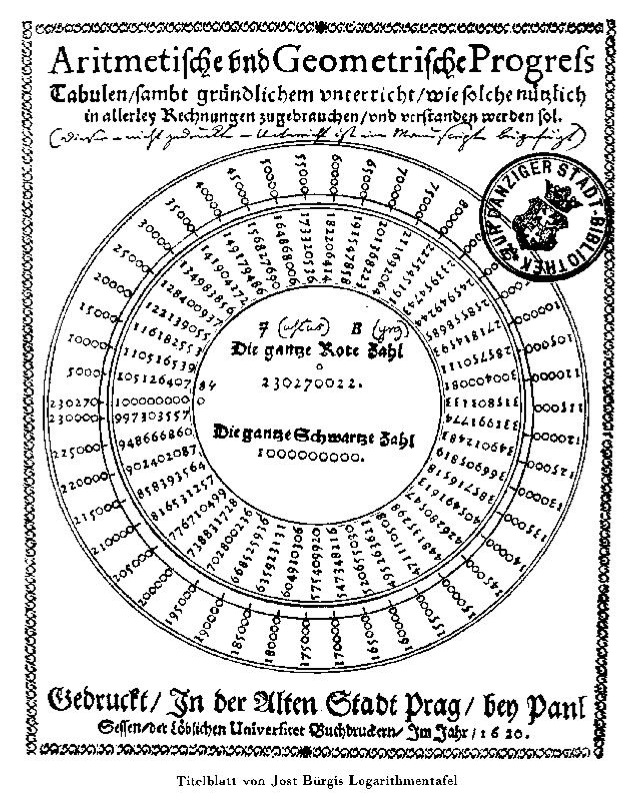
\includegraphics[width=0.37\textwidth]{pictures/logarithmentafel}
  \end{center}
\end{wrapfigure}
Wir möchten also eine gegebene Gleichung mit Variable im Exponenten lösen können. Dafür gehen wir von den bereits bekannten Exponentialfunktionen aus. Die Exponentialfunktion
$$f(x)=b^x$$
ist für $0<b<1$ streng monoton fallend und für $b>1$ streng monoton wachsend. Deshalb existiert eine Umkehrfunktion $f^{-1}$. Diese nennt man Logarithmusfunktion zur Basis $b$ und bezeichnet sie mit $\log_b$.

\uebh{}{
Wie lautet das Kriterium für die Existenz einer Inversfunktion? Nenne eine Funktion, welche keine Inversfunktion besitzt.
} 

\uebh{}{
Zeichne die Funktion $f(x)=2^x$ und den Graphen der Inversfunktion $f^{-1}(x)=\log_2(x)$. Siehst du den bekannten graphischen Zusammenhang zwischen Funktion und Inversfunktion?
}

\uebh{}{
Betrachte den Graphen der Funktion $f(x)=\log_2(x)$ in einem Koordinatensystem.
\begin{enumerate}[a)]
\item Verschiebe den Graphen in positiver x-Richtung um 2 Einheiten.
\item Spiegle  den Graphen an der x-Achse.
\end{enumerate}
Gib jeweils die Gleichung der Bildkurve an.
}

\begin{wrapfigure}{r}{0.3\textwidth}
\begin{center}
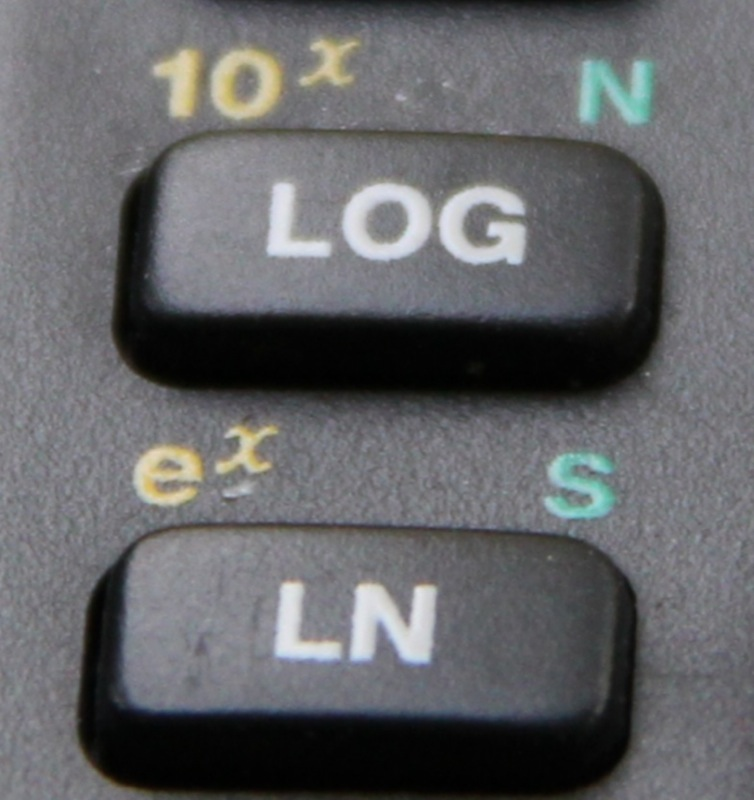
\includegraphics[width=0.2\textwidth]{pictures/logln}
\end{center}
\end{wrapfigure}
Mit der \fbox{log}-Taste kann man Werte von Variablen in
Exponenten bestimmen. Um sie korrekt
einsetzen zu können, wollen wir erst definieren, was wir unter einem Logarithmus verstehen wollen. Die Definition entspricht grundsätzlich einer Regel zum Umschreiben von Exponentialfunktionen.
\begin{cdef}[Logarithmus]{}
  Unter
\marginnote{
\qrcode{
https://www.youtube.com/watch?v=3LtdUV1l33g}
}
  dem \emph{Logarithmus} von $y$ zur Basis $b$, geschrieben
  $$\log_b{y},$$ versteht man diejenige Zahl, welche als Exponent
  der Basis $b$ den Wert $y$ ergibt. Mathematisch notiert wird diese
  Aussage übersichtlich:
  $$x=\log_b{y}\quad \Leftrightarrow \quad b^x=y.$$
  $y$ nennt man \emph{Numerus} und $b$ \emph{Basis} des Logarithmus.
\end{cdef}

\begin{bem}
  Bei Betrachtung obiger Äquivalenz wird klar, dass der Logarithmus nur für $y,b\in\D{R}^+$ und $b\neq1$
  definiert ist.
\end{bem}

\uebh{}{
Überlege kurz, welche Probleme entstünden, wenn man $y,b\in\mR$ zulassen würde.
}

\begin{bsps}
\ \\[-3ex]
  \begin{itemize}
    \item Den Logarithmus von $y$ zur Basis $b$ finden, ist gleichwertig
    mit der Beantwortung der Frage: \glqq $b$ hoch was gibt $y$?\grqq
    \item $\log_2{8}=3$: Der Logarithmus von $8$ zur Basis $2$ ist $3$,
    denn $2^3=8$.
    \item $\log_{10}{100}=2$, weil $10^2=100$.
    \item $\log_{\frac{1}{3}}{\frac{1}{9}}=2$, da
    $(\frac{1}{3})^2=\frac{1}{9}$.
  \end{itemize}
\end{bsps}

\uebh{}{
Bestimme

\begin{minipage}{0.49\textwidth}
\begin{enumerate}[a)]
\item $\log_{10}1000$, $\log_{10}1000000$, $\log_{10}10^6$, $\log_{10}10^{837}$
\item $\log_{10}0.1$, $\log_{10}0.01$, $\log_{10}\frac{1}{10}$, $\log_{10}\frac{1}{100}$
\end{enumerate}
\end{minipage}
\begin{minipage}{0.49\textwidth}
\begin{enumerate}[a)]
\setcounter{enumi}{2}
\item $\log_{2}4$, $\log_{2}1024$, $\log_{2}\frac{1}{4}$, $\log_{2}\frac{1}{512}$
\item $\log_{e}1$, $\log_{e}e$, $\log_{e}e^3$, $\log_{e}\frac{1}{e^4}$
\end{enumerate}
\end{minipage}
}
Der folgende Satz folgt direkt aus der Definition und
bringt meine saloppe Formulierung aus dem obigen Beispiel auf den
Punkt.
\begin{csatz}[Exponenten-Eigenschaft]{}
  Jeder Logarithmus ist ein Exponent.
\end{csatz}

\begin{proof}[Beweis]
trivial
\end{proof}

\subsection{Übliche Bezeichnungen und Schreibweisen}

Erstens werde ich anstelle von $\log_b(y)$ nun oft $\log_b(x)$ schreiben. Das $y$ habe ich verwendet, um klar darzustellen, dass der Logarithmus $x=\log_b(y)$ die Umkehrfunktion einer Exponential\-funktion $y=b^x$ ist. In andern Worten wird hier der Schritt \glqq Vertauschung der Variablen\grqq --- der ja beim Algorithmus zur Bestimmung von Inversfunktionen als letzter erfolgt ---  schliesslich vorgenommen.
Zweitens kommt als Basis $b$ des Logarithmus
$$\log_bx$$
oft eine der drei Zahlen $2$, $e$ (Euler'sche Zahl) oder $10$ vor. Deshalb legt man folgende,
kürzere Schreibweisen fest:
\begin{itemize}
  \item $\log_{10}x=\log{x}=\lg x$\hfill(10$^{\text{er}}$ Logarithmus)
  \item $\log_\mathrm{e}{x}=\ln{x}$\hfill(Logarithmus naturalis)
  \item $\log_2{x}=\lb{x}$\hfill(Logarithmus dualis)
\end{itemize}
\begin{bem}
  Die \fbox{log} - Taste auf dem Taschenrechner ist also der
  Logarithmus zur Basis $10$.
\end{bem}
Drittens werde ich oft die Klammer um den Numerus weglassen, falls das Argument der Logarithmusfunktion klar ersichtlich ist. So wie das unter \glqq Zweitens\grqq\ bereits geschehen ist. Manchmal schreibe ich den Numerus in Klammer, um deutlich zu
kennzeichnen, was alles zum Logarithmus gehört. Zum Beispiel
$$\log_{3.5}(4x^3+2x-1).$$

\uebh{}{
Lasse von \geogebralink\  folgende Logarithmusfunktionen zeichnen.
\begin{itemize}
\item $f(x) = \log (x)$
\item $g(x) = \ln (x)$
\end{itemize}
}

\begin{figure}
\begin{center}
\definecolor{qqzzww}{rgb}{0,0.2,1}
\definecolor{zzqqtt}{rgb}{0.6,0,0.4}
\definecolor{cqcqcq}{rgb}{0.75,0.75,0.75}
\begin{tikzpicture}[line cap=round,line join=round,>=triangle 45,x=0.8cm,y=0.8cm]
\draw [color=cqcqcq,dash pattern=on 3pt off 3pt, xstep=1.6cm,ystep=1.6cm] (-1.4,-4.86) grid (11.72,4.7);
\draw[->,color=black] (-1.4,0) -- (11.72,0);
\foreach \x in {1,2,3,4,5,6,7,8,9,10,11}
\draw[shift={(\x,0)},color=black] (0pt,2pt) -- (0pt,-2pt) node[below] {\footnotesize $\x$};
\draw[color=black] (11.38,0.08) node [anchor=south west] { $x$};
\draw[->,color=black] (0,-4.86) -- (0,4.7);
\foreach \y in {-4,-3,-2,-1,1,2,3,4}
\draw[shift={(0,\y)},color=black] (2pt,0pt) -- (-2pt,0pt) node[left] {\footnotesize $\y$};
\draw[color=black] (0.1,4.3) node [anchor=west] { $y$};
\clip(-1.4,-4.86) rectangle (11.72,4.7);
\draw[smooth,samples=100,domain=0.01:11.72, line width=0.5mm] plot(\x,{ln(\x)});
\draw[color=zzqqtt, smooth,samples=100,domain=0.01:11.72, line width=0.35mm] plot(\x,{ln(\x)/ln(2)});
\draw[color=qqzzww, smooth,samples=100,domain=0.01:11.72, line width=0.35mm] plot(\x,{ln(\x)/ln(10)});
\draw[color=black] (9.5,1.8) node {$\ln$};
\draw[color=zzqqtt] (9.5,2.8) node {$\lb$};
\draw[color=qqzzww] (9.5,0.5) node {$\log$};
\end{tikzpicture}
\end{center}
\caption{Die Graphen von $\ln(x)$, $\log(x)$, und $\lb(x)$}
\end{figure}

\uebh{}{
Die Funktion
$$f(x)=\log_b(x)$$
ist für $b >1$ eine monoton wachsende Funktion. Allerdings ist dieses Wachstum sehr langsam. Um einen Eindruck davon zu bekommen, denke man sich ein Koordinatensystem, dessen $x$-Achse mehrere Äquatorumfänge lang ist.
Die Einheit sei $\unit[1]{cm}$. Überprüfe die Abbildung \ref{logvsaequator} für den Graphen von $\log(x)$ und zeichne die Werte von zwei weiteren \glqq Erdumrundungen\grqq\ in Abbildung \ref{logvsaequator} auf Seite \pageref{logvsaequator} ein.

\begin{figure}
\begin{center}
\definecolor{cqcqcq}{rgb}{0.75,0.75,0.75}
\begin{tikzpicture}[line cap=round,line join=round,>=triangle 45,x=0.6cm,y=0.6cm]
\draw [color=cqcqcq,dash pattern=on 2pt off 2pt, xstep=1.2cm,ystep=1.2cm] (-0.84,-0.62) grid (12.86,11.66);
\draw[->,color=black] (-0.84,0) -- (12.86,0);
\foreach \x in {,1,2,3,4,5,6,7,8,9,10,11,12}
\draw[shift={(\x,0)},color=black] (0pt,2pt) -- (0pt,-2pt) node[below] {\footnotesize $\x$};
\draw[color=black] (12.52,0.08) node [anchor=south west] { x};
\draw[->,color=black] (0,-0.62) -- (0,11.66);
\foreach \y in {,1,2,3,4,5,6,7,8,9,10,11}
\draw[shift={(0,\y)},color=black] (2pt,0pt) -- (-2pt,0pt) node[left] {\footnotesize $\y$};
\draw[color=black] (0.1,11.26) node [anchor=west] { y};
\clip(-0.84,-0.62) rectangle (12.86,11.66);
\draw[smooth,samples=100,domain=0.0:12.86] plot(\x,{9.6});
\draw[smooth,samples=100,domain=0.2:12.86] plot(\x,{ln(\x)/ln(10)});
\draw[color=black] (6,9) node {nach der 1. Erdumrundung};
\end{tikzpicture}
\end{center}
\caption{Log der Äquator-Vielfachen}\label{logvsaequator}
\end{figure}
}

\uebh{}{
  Berechne mit dem TR folgende Logarithmen, und kontrolliere deine Berechnung, indem du $10$ \glqq hoch\grqq\ dein jeweiliges Resultat eintippst.\\
  
  \begin{minipage}{0.49\textwidth}
    \begin{enumerate}[a)]
      \item $\log{7}$
      \item $\log{1001}$
      \item $\log{1024}$
    \end{enumerate}
  \end{minipage}
  \begin{minipage}{0.49\textwidth}
    \begin{enumerate}[a)]\addtocounter{enumi}{3}
      \item $\log{0.101}$
      \item $\log{10^{-23}}$
      \item $\log{0.5}$
    \end{enumerate}
  \end{minipage}
}

\subsection{Rechenregeln}

\subsection{Die Logarithmensätze}
Es folgen vier Logarithmenregeln. Die erste ist hilfreich beim
Eintippen in den Taschenrechner. Die letzte beschreibt, wie man
Gleichungen nach einer im Exponenten stehenden Variablen auflöst. Damit werden Sie dann in der Lage sein, für unser Ausgangsproblem auf Seite 1 den exakten Wert von $t$ zu bestimmen.

Die erste Regel besagt, dass jeder Logarithmus zu einer beliebigen Basis $b$ als Quotient von
Logarithmen zu einer beliebigen Basis $n$ geschrieben werden kann.
\begin{csatz}[Basiswechsel]{\label{satz:logtr}}\label{satz:logtr}
\marginnote{
\qrcode{
https://www.youtube.com/watch?v=79ax8cwhggk}
}
  $$\log_b{x} = \frac{\log_n{x}}{\log_n{b}}$$
\end{csatz}
Um diesen Satz zu beweisen, brauchen wir eine der folgenden drei Rechenregeln,
die leicht mit der Definition nachgewiesen werden können.\pagebreak

\begin{csatz}[Rechenregeln für Logarithmen]{}
Es
\marginnote{
\qrcode{
https://www.youtube.com/watch?v=xzwY11unPRI}
}
gilt
\begin{align}
  \log_b{(u\cdot v)}&=\log_b{u} + \log_b{v}\\[1ex]
  \log_b{\dfrac{u}{v}}&=\log_b{u} - \log_b{v}\\[1ex]
  \log_b{u^n}&=n\cdot\log_b{u}
\end{align}
\end{csatz}

\begin{proof}[Beweis]
  Nach Definition; also Übung. Hinweis: Erinnere dich daran, dass ein Logarithmus die Inversfunktion einer Exponentialfunktion ist und daher die Gesetze ähnlich zu den Potenzgesetzen sein müssen.
\end{proof}
\begin{proof}[Beweis zu Satz \ref{satz:logtr}]
  Es sei $\log_b{x} = y$, also
  $b^y=x$. Diese Exponentialgleichung logarithmieren wir auf beiden Seiten
  $$\log_n{b^y}=\log_n{x}.$$ Mit der dritten Logarithmenregel folgt dann
  $y\cdot\log_n{b}=\log_n{x}\q \Leftrightarrow\q
  y=\frac{\log_n{x}}{\log_n{b}}$
  Daraus folgt unmittelbar die Behauptung.
\end{proof}

\subsection{Graphen von Logarithmenfunktionen}
Sie haben ein
paar Graphen anhand von Wertetabellen oder mit \geogebralink\  gezeichnet.

\uebh{}{
  Skizziere die Graphen der Funktionen $f(x)=\log_e(x)$ und
  $g(x)=\log_{\frac{1}{e}}(x)$ in ein und dasselbe
  Koordinatensystem. Was fällt auf?
}

\uebh{}{
Skizziere die Graphen der Funktionen $f(x)=\ln x$ und $g(x)=e^x$ in ein und dasselbe Koordinatensystem. Was fällt auf? Erkläre das Ergebnis.
}

\uebh{}{
Vereinfache
$e^{\ln 2}$, $\ln(e^2)$, $e^{\ln(x)}$, $\ln(e^x)$?
}

\begin{csatz}[Eigenschaften der Logarithmusfunktion]{}
  Graphen von Logarithmusfunktionen haben folgende Eigenschaften:
  \begin{itemize}
    \item Sie gehen alle durch den Punkt $\point{1}{0}$.
    \item Die Graphen von $f(x)=\log_b{(x)}$ und
    $g(x)=\log_{\frac{1}{b}}{(x)}$ sind achsialsymmetrisch bezüglich
    der x-Achse.
  \end{itemize}
\end{csatz}

\begin{proof}[Beweis]
  Wir betrachten eine beliebige Logarithmusfunktion $f(x)=\log_b(x)$.
  Also $f(1)=\log_b(1)$ genau dann, wenn $b^{f(1)}=1$, dh. $f(1)=0$ und
  der erste Punkt ist bewiesen.

Um den zweiten Punkt zu verifizieren betrachten wir:
\begin{align*}
g(x)&=\log_{\frac{1}{b}}(x)=\log_{b^{-1}}(x)=\frac{\log_b (x)}{\log_b (b^{-1})}\\
&=\frac{\log_b (x)}{-\log_b (b)}=-\log_{b}(x)=-f(x).
\end{align*}
Also sind
  die Graphen von $f(x)$ und $g(x)$
  symmetrisch bezüglich der x-Achse.
\end{proof}

\uebh{}{
  Gegeben sei die natürliche Exponentialfunktion
  $$f(x)=\mathrm{e}^x$$
  \begin{enumerate}[a)]
    \item Zeichne den Graphen von $f$ und spiegle diesen an der
    Winkelhalbierenden durch den 1. und 3. Quadranten. Überlege, dass durch die Spiegelung der Graph einer neuen Funktion $g$ entsteht.
    \item Bestimme die Funktionswerte von $g$ an den Stellen
    $\mathrm{e}$, $\mathrm{e}^2$, $\mathrm{e}^{-1}$ und $\sqrt{\mathrm{e}}$.
    \item Gib die Funktion $g$ an.
  \end{enumerate}
}

Schliesslich halten wir noch fest, was wir zu Beginn einfach in den Raum geworfen haben:

\begin{csatz}[Log als Inversfunktion von Exp]{}
  Jede Logarithmusfunktion ist die Inverse einer Exponentialfunktion
  und vice-versa.
\end{csatz}

\begin{proof}[Beweis]
  Wir bestimmen die Inversfunktion einer beliebigen Exponentialfunktion:
  $$y=b^x\q \Leftrightarrow\q x=\log_b(y).$$ Variablen umbenennen
  und die Inversfunktion mit $f^{-1}$ bezeichnen:
  $f^{-1}(x)=\log_b(x).$ Die Umkehrung gilt ebenfalls, weil wir
  ausschliesslich Identitäten und Äquivalenzen verwendet haben.
\end{proof}

\subsection{Weitere Anwendungen}
  Logarithmen kann man benutzen, um Zahlen zu berechnen, welche
  ausserhalb der Kapazität des TRs liegen.
\begin{bsp}
  Wir wollen $x=2^{4000}$ berechnen. Eingetippt in den TR erhalten wir
  leider nur die obere Kapazitätsgrenze; der TR ist überfordert.

  Wir helfen der Rechenmaschine etwas nach, indem wir sie instrumentalisieren:
  $$\log(x)=\log(2^{4000})=4000\cdot\log(2)= 1204.1199 $$
  Das bedeutet
\begin{align*}
x&=10^{1204.1199}=10^{1204+0.1199}\\
&=10^{0.1199}\cdot10^{1204}=1.318\cdot10^{1204}
\end{align*}
\end{bsp}

\uebh{}{
  Berechne $$9^{(9^9)}.$$
}

\uebh{}{
  Der \unit{pH}-Wert ist ein Mass für die H$_3$O$^+$-Konzentration einer Lösung. Es gilt
  $$\unit{pH} = -\log{H}$$ wobei $H$ die Konzentration von H$_3$O$^+$
   in \unitfrac{mol}{l} bezeichnet.
   \begin{figure}
\begin{center}
  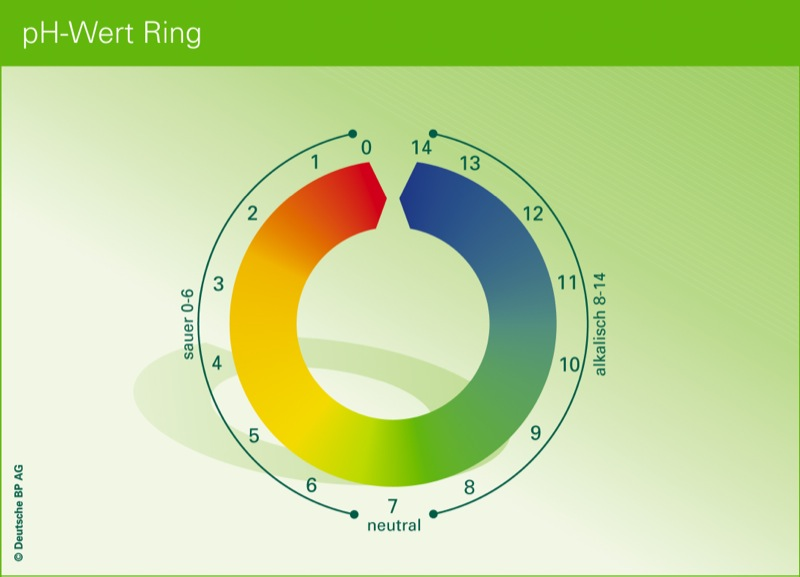
\includegraphics[width=0.618\textwidth]{pictures/phring}
  \caption{PH-Ring}
\end{center}
\end{figure}  
  \begin{enumerate}[a)]
    \item Für Tomaten ist $H=\unitfrac[6.3\cdot10^{-5}]{mol}{l}$,
    für Milch $H=\unitfrac[4\cdot10^{-7}]{mol}{l}$. Berechne
    die zugehörigen \unit{pH}-Werte.
    \item Welcher \unit{pH}-Wert hat eine Lösung mit
    $H=\unitfrac[0]{mol}{l}$?
  \end{enumerate}
}

\uebh{}{
  Die Lautstärke $L$ eines Geräuschs von der Intensität $I$ ist
  definiert durch $$L=\unit[10\cdot\log\left(\frac{I}{I_0}\right)]{dB}.$$
  \unit{dB}
  steht für Dezibel, nach dem amerikanischen Ingenieur \textsc{Graham Bell}
  (1847--1922); dem Erfinder des Telefons. $I_0$ bedeutet die Intensität
  eines Geräuschs, das vom menschlichen Ohr gerade noch wahrgenommen
  werden kann.
  \begin{enumerate}[a)]
    \item Die Geräuschintensität normaler Unterhaltung ist etwa eine
    Million mal so gross wie $I_0$. Welchem Dezibel-Wert entspricht
    das?
    \item Eine Intensitätszunahme von $10$ Dezibel empfindet das
    menschliche Ohr als Verdoppelung der Lautstärke. Welcher
    Intensitätszunahme in Prozent entspricht dies?
    \item Ein Düsenflugzeug entwickelt beim Start eine Intensität
    von $10^{13}I_0$. Dezibel-Werte von mehr als $\unit[90]{dB}$
    gelten als gehörschädigend; ist es die angegebene Intensität?
  \end{enumerate}
}
\begin{figure}
\centering
    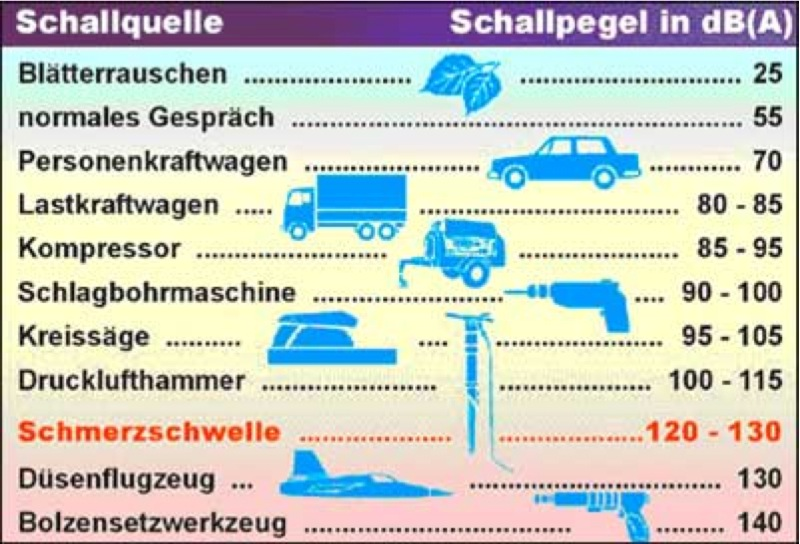
\includegraphics[width=0.618\textwidth]{pictures/dbtabelle}
    \caption{Schallpegel-Tabelle}
 \end{figure}

\uebh{}{
Die Stärke von Erdbeben $R$ gibt man durch Werte der sogenannten
    \emph{Richter-Skala} an. Diese ist definiert durch
    $$R=\log\left(\frac{B}{B_0}\right),$$ wobei $B_0$ die Intensität
    eines gerade noch wahrnehmbaren Bebens bezeichnet.

  \begin{enumerate}[a)]
    \item Das Beben von San Francisco im Jahr 1906 hatte eine
    Intensität von $B=B_0\cdot10^{8.25}$. Welchem Wert auf der
    Richter-Skala entspricht dies?
    \item Welche Intensitätsänderung bedeutet eine Zunahme von $1$
    auf der Richterskala?
  \end{enumerate}  
    \begin{figure}
  \centering
    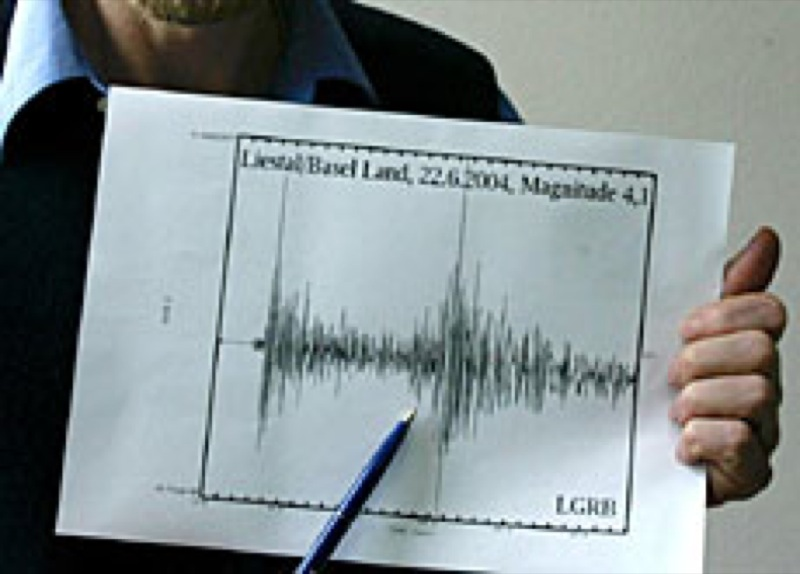
\includegraphics[width=0.618\textwidth]{pictures/erdbebenbasel}\\
    \caption{Aufzeichnung des Erdbebens von Basel vom 22.~Juni 2004}
  \end{figure}
  
}

\subsection{Gleichungen mit Variablen im Exponenten}
Die Lösung unseres Ausgangsproblems, die
Bestimmung von Variablen in Exponenten, soll an einem Beispiel
vorgeführt werden.
\begin{bsp}
  Wir lösen die Gleichung $$6^{x-1}=10$$ nach $x$ auf. Dies können
  wir auf zwei Arten tun.
  \begin{enumerate}
    \item Mit Logarithmieren auf beiden Seiten:
    \begin{align}
      \log{6^{x-1}}&=\log{10} \tag{Regel (3)}\\
      (x-1)\cdot\log{6}&= 1 \tag{$\div\log{6}$}\\
      x-1 &= \frac{1}{\log{6}} \tag{$+1$}\\
      x &= \frac{1}{\log{6}} + 1 \approx 2.285 \notag
    \end{align}
    \item Mit der Definition:
    \begin{align}
      6^{x-1}=10\q \Leftrightarrow\q x-1 &= \log_6{10} \tag{Satz \ref{satz:logtr}}\\
      x-1 &= \frac{\log{10}}{\log{6}} \tag{$+1$}\\
      x &= \frac{1}{\log{6}} + 1 \notag
    \end{align}
  \end{enumerate}
  Kontrolle: $$6^{2.285-1} \approx 10 \qq \checkmark$$
\end{bsp}

\uebh{}{
  Löse nach $x$ auf: $$2000\cdot1.025^x = 3750$$
}

\uebh{}{
  Stelle drei Gleichungen auf, bei denen die Variable im
  Exponenten vorkommt. Löse diese und überprüfe deine Resultate durch
  Einsetzen in die ursprüngliche Gleichung.
}

\uebh{}{
Nach UNO-Angaben lebten 1988 auf der Erde 5113 Millionen Menschen; die jährliche Wachstumsrate betrug 1.7\%. Wann wird unter der Annahme, dass diese Zuwachsrate konstant bleibt, jedem Menschen nur noch ein Stehplatz von $\unit[\frac{1}{4}]{m^2}$ zur Verfügung stehen? (Die Landfläche beträgt 29\% der Erdoberfläche.)
}

\uebh{}{
Der Landesindex der Konsumentenpreise betrug im September 1981 94.5 Punkte und im September 1987 109.7 Punkte.
\begin{enumerate}[a)]
\item Berechne den Landesindex im September 1989
unter der Annahme von exponentiellem Wachstum.
\item Wann wird der Landesindex 130 Punkte erreichen?
\end{enumerate}
}

%Spannung]
%Die Spannung $U$ (in Volt) einer 12-Volt-Batterie
%beträgt während des Einschaltvorganges im Zeitpunkt $t$ (in Sekunden)
$$U(t) = a(1 - b^t)$$
%Man misst $U(0.1) = 10.22$.
%\begin{enumerate}[a)]
%\item Bestimme die Parameter $a$ und $b$.
%\item Wie gross ist die Spannung nach $0.2$ Sekunden?
%\item Wann beträgt die Spannung 6 Volt?
%\end{enumerate}
%}

\uebh{}{
Beim radioaktiven Zerfall wird meistens die sogenannte Halbwertszeit angegeben. Die Halbwertszeit ist die Zeit, in der die Hälfte der zu Beginn vorhandenen Atome zerfallen ist.
%\begin{enumerate}[a)]
%\item Berechne die Halbwertszeit für Strontium 89, für das die Zerfallsfunktion die Form
%$$N(t)=N_0\cdot0.98636808^t$$
%hat (t in Tagen).
Für Uran 239 beträgt die Halbwertszeit $T_{\nicefrac{1}{2}}=23.5$
Minuten. Stelle die Gleichung der Zerfallsfunktion auf, wenn zu Beginn $N_0$ Atome vorhanden sind.
%\end{enumerate}
}

\uebh{}{
In lebenden Organismen besteht Kohlenstoff aus stabilen Atomkernen sowie einem Anteil ($3\cdot10^{-8}\%$) aus radioaktiven Atomkernen C$_{14}$, die durch kosmische Strahlung entstehen. Sobald ein organischer Stoff stirbt, nimmt der C$_{14}$-Anteil mit einer Halbwertszeit von 5736 Jahren exponentiell ab.
\begin{enumerate}[a)]
\item Im Jahre 1960 stellte man in der Leinwand einer altägyptischen Königsmumie einen C$_{14}$-Anteil von $1.75\cdot10^{-8}\%$ fest. Datiere auf hundert Jahre genau.
\item 1950 wurde in der Höhle von Lascaux (Frankreich) Holzkohlenreste mit einem C$_{14}$-Anteil von $0.435\cdot10^{-8}\%$ gefunden. Berechne das Alter dieser Holzkohle.
\end{enumerate}
}

\uebh{}{
In der Informationstheorie versteht man unter dem Informationsgehalt $H$ eines Ereignisses mit der Wahrscheinlichkeit $p$ den Logarithmus von $\frac{1}{p}$ zur Basis 2.
$$H = \log_2\frac{1}{p}\q\text{(Einheit: 1 bit)}$$
Welche Wahrscheinlichkeit gehört zum Informationsgehalt $0, 1,0.5,5, 10.2$ bit?

Eine Münze wird viermal geworfen. Berechne den Informationsgehalt der Ereignisse
\begin{enumerate}[a)]
\item nie Kopf,
\item genau einmal Kopf,
\item genau zweimal Kopf,
\item genau dreimal Kopf
\item viermal Kopf.
\end{enumerate}
}

\subsection{Die Euler'sche Zahl}
Die geeignetste Basis für eine Exponentialfunktion
$$f(x)=b^x$$
ist die Zahl $\mathrm{e}$, eine Zahl, die in vielen Anwendungen vorkommt. Der Buchstabe $\mathrm{e}$ wurde zu Ehren des in Riehen geborenen Mathematikers \textsc{Leonhard Euler} (1707-1783) gewählt. Wie $\pi$ ist die Euler'sche Zahl irrational, und ihre Dezimaldarstellung beginnt mit
$$\mathrm{e}  =  2.71828182845904523536028747135266\dots$$

\begin{figure}
\begin{center}
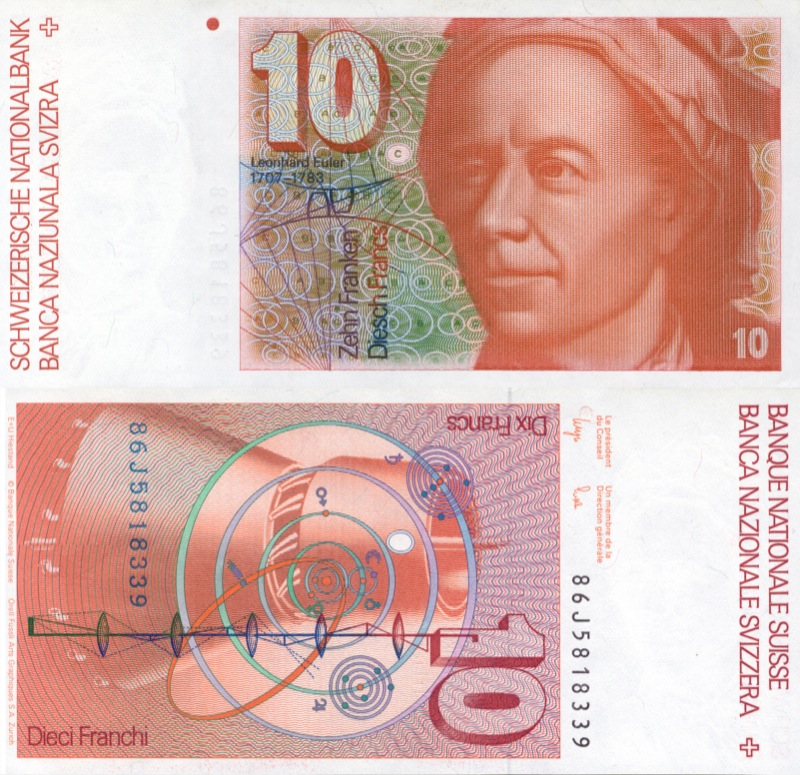
\includegraphics[width=0.618\textwidth]{pictures/euler}
\end{center}
\caption{10-Franken Note alter Serie: Leonard Euler}
\end{figure}

Was es mit der Zahl $e$ auf sich hat, können wir an dieser Stelle nur zu einem kleinen Teil erfahren, denn ihre Bedeutung wird erst nach und nach mit fortschreitendem Stoff klarer werden. Eine Möglichkeit, die Zahl $\mathrm{e}$ kurz und bündig zu charakterisieren, ist diese:
\begin{quote}
$\mathrm{e}$ ist die einzige positive Zahl, für die
$$\mathrm{e}^x\geq1+x\q\forall x\in\mR$$
\end{quote}

\uebh{}{
Zeichne mit dem TR $\mathrm{e}^x$ und $x+1$.
}

\uebh{}{
Zeichne mit dem TR $\mathrm{e}^x$, $2^x$ und $3^x$ und betrachte einen kleinen Ausschnitt um $\point{0}{1}$.
}

Eine weitere schöne Eigenschaft ist folgende.
\begin{bem}
Alle Exponentialfunktionen $b^x$ schneiden die $y$-Achse im Punkt $\point{0}{1}$. Sucht man für eine Exponentialfunktion $b^x$ eine Basis $b$ so, dass die Steigung des Graphen beim Schnittpunkt mit der $y$-Achse exakt $45^\circ$, also $1$, beträgt, dann folgt $b=\mathrm{e}$.
\end{bem}

Obwohl die bisherige Argumentation von einem strengen mathematischen Gesichtspunkt aus betrachtet  zu schlampig ist, geben wir uns mit ihr zufrieden. Auch ein genauerer Beweis liefert dasselbe Resultat.

Um die Basis Euler'sche Zahl zu berechnen, gehen wir folgendermassen vor: Wir wählen ein positives $x$ und betrachten jene Basis $b$, für die
$$b^x=1+x$$
oder, nach $b$ aufgelöst
$$b=(1+x)^{\frac{1}{x}}$$
ist. Dies ist genau jene Basis, für die der Graph von $b^x$ die Gerade $1+x$ in einem Punkt mit der (positiven) x-Koordinate $x$ schneidet. Wenn wir nun $x$ immer kleiner machen ($x\to0$), wird $b$ immer näher an $\mathrm{e}$ heran rücken.
Wir berechnen sinngemäss
$$\left(1+\frac{1}{n}\right)^n$$
für grosse natürliche Zahlen $n$, also $n\to\infty$.

\begin{table}
\begin{center}
\scalebox{1.1}{
\begin{tabular}{|c|c|}
\hline
\rowcolor{lightyellow}\spaltenheight    $n$ & $\left(1+\frac{1}{n}\right)^n$\spaltensep\hline\hline
\rowcolor{Gray}\spaltenheight 1 & 2\spaltensep\hline
\rowcolor{lightyellow}\spaltenheight    2 & 2.25\spaltensep\hline
\rowcolor{Gray}\spaltenheight 10 & 2.59\dots\spaltensep\hline
\rowcolor{lightyellow}\spaltenheight    100 & 2.70\dots\spaltensep\hline
\rowcolor{Gray}\spaltenheight 1000 & 2.716\dots\spaltensep\hline
\rowcolor{lightyellow}\spaltenheight    100000 & 2.71826\dots\spaltensep\hline
\rowcolor{Gray}\spaltenheight 100000000 & 2.71828\dots\spaltensep\hline
\end{tabular}
}
\end{center}
\caption{Approximation an $\mathrm{e}$}
\end{table}

\begin{cdef}[Euler'sche Zahl]{}
Es
\marginnote{
\qrcode{
https://www.youtube.com/watch?v=0NK4BMpqd2Q}
}
ist denkbar, als Definition für die Euler'sche Zahl
$$\mathrm{e}:=\lim_{n\to\infty}\left(1+\frac{1}{n}\right)^n=2.718281828\dots$$
zu verwenden.
\end{cdef}

\begin{cdef}[Natürliche Exponentialfunktion und logarithmus naturalis]{}
Die entsprechende Exponentialfunktion
$$\mathrm{exp}(x)=\mathrm{e}^x$$
bezeichnet man als die \emph{natürliche Exponentialfunktion}.

Die entsprechende Logarithmusfunktion, also die Umkehrfunktion von $x\mapsto \mathrm{e}^x$, wird \emph{natürliche Logarithmusfunktion} genannt:
$$\mathrm{exp}^{-1}(x)=\log_\mathrm{e}(x)=:\ln(x)$$
\end{cdef}

\begin{bem}
Der Taschenrechner stellt mit speziellen Tasten sowohl die Funktionswerte $\mathrm{e}^x$ als auch die Funktionswerte $\ln(x)$ zur Verfügung.
\end{bem}

\begin{bem}
Fortgeschrittene Rechner verwenden selbstverständlich als Basis einer Exponentialfunktion $\mathrm{e}$ und bezeichnen den $\ln$ oft als $\log$.

Später werden wir in erster Linie nur noch diese beiden Funktionen verwenden, da sich alle anderen Exponential- und Logarithmusfunktionen auf diese beiden Funktionen zurückführen lassen. Diese schöne Tatsache wollen wir mit den beiden nächsten Übungen untermauern.
\end{bem}

\uebh{}{
Stelle die Exponentialfunktion $f(x)=3.5\cdot2^x$ als natürliche Exponentialfunktion der Form
$$f(x)=a\cdot \mathrm{e}^{cx}$$
dar.
}

%\uebh{}{[Es gibt nur eine Basis\dots]
%Überlege dir, dass jede Exponentialfunktion $f(t)=a\cdot b^t$
%sich in die Form
%$$f(t)=d\cdot \mathrm{e}^{ct}$$
%umwandeln lässt.

%Finde eine Formel für die Parameter $c$ und $d$ bei der natürlichen Exponentialfunktion, wenn die Parameter $a$ und $b$ gegeben sind.
%}

\uebh{}{
Für die Zeit während der Ausbreitung einer Epidemie kann man die Anzahl der nach $t$ Tagen infizierten Individuen durch die folgende Modellfunktion angeben:
$$N(t)=\frac{M}{1+c\mathrm{e}^{-at}}$$
Für eine bestimmte Epidemie seien $M= 1000$, $c=999$
und $a=0.4$.
\begin{enumerate}[a)]
\item Wie viele Individuen sind nach 0, 10, 20, 30 Tagen infiziert?
\item Nach wie vielen Tagen sind 200, 500, 950 Individuen infiziert?
\item Zeichne den Graphen der Funktion.
\end{enumerate}
}

%\uebh{}{[Forellen]
%In einer Forellenzuchtanstalt wurde bei gleichartigen Forellen die jeweils nach $t$ Monaten erreichte durchschnittliche Länge $\unit[L]{cm}$ gemessen. Aus den Messungen ergab sich das \glqq Wachstumsgesetz\grqq:
%$$L(t) =25(1- \mathrm{e}^{-0.25t})$$
%\begin{enumerate}[a)]
%\item Berechne die Länge nach 0, 4, 8 Monaten.
%\item Wann waren die Forellen etwa $\unit[10,20]{cm}$ lang?
%Wann werden sie $\unit[25]{cm}$ lang sein?
%\end{enumerate}
%}

\cleardoublepage

\end{document}